\documentclass[12Pt]{article}
%\documentclass[11pt,a4paper]{article}
%\documentclass{article}
\usepackage{amssymb,euscript,latexsym,amsmath}
\usepackage{graphicx}
\usepackage[dvips]{epsfig}
%\usepackage{color}
%\usePackage{Pdfsync}
\usepackage{epstopdf}
\usepackage[ ]{algorithm2e}
\usepackage{hyperref}
\usepackage{subfigure}
\usepackage{hyperref}
\usepackage{multirow}
\usepackage{color,soul}
\usepackage{color}
\usepackage{xcolor}
\usepackage{booktabs}
\usepackage{appendix}
\usepackage[numbers]{natbib}
\hypersetup{
 pdftitle={},
 pdfauthor={Eva Kanso},
 pdfsubject={Curriculum Vitae},
 pdfkeywords={},
 pdfpagemode=UseThumbs,
 baseurl={http://www-rcf.usc.edu/~kanso/},
%  pagebackref=true,
% turn off boxes around references
 colorlinks=true,
 linkcolor=black,
 anchorcolor=black,
 citecolor=black,
 filecolor=black,
 menucolor=black,
 urlcolor=blue,
 bookmarksopen=false,
}
% end hyperref stuff
\DeclareGraphicsRule{.tif}{png}{.png}{`convert #1 `dirname #1`/`basename #1 .tif`.png}


\textwidth = 6.5 in
\textheight = 9 in
\oddsidemargin = -0.0 in %0.2in %0.75 in
\evensidemargin = -0.1 in
\topmargin = 0.0 in
\headheight = 0.0 in
\headsep =  0.0 in
\parskip =  0in %\baselineskip
\parindent = 0.4in

\newcommand{\sh}[1]{\textcolor{red}{sh: #1}}
\newcommand{\shnote}[1]{\marginpar{\tiny\textcolor{blue}{sh: #1}}}

\usepackage{caption2}%\itshape
\renewcommand{\captionfont}{\footnotesize}
\renewcommand{\captionlabelfont}{\upshape}


\newcommand{\rv}[1]{\textcolor{blue}{#1}}
%\newcommand{\rv}[1]{\textcolor{RedOrange}{#1}}

\DeclareGraphicsExtensions{.eps,.ps,.pdf}

\bibliographystyle{plain}
%-----------------------------


%\setlength{\parindent}{0em}

\begin{document}


\begin{center}
{\bf \Large{CSCI 596 Course project}} \\[2ex]
{\bf \Large{A parallel reinforcement learning framework}} \\[2ex]
{Kishore Ganesh, Qiongao Liu, Yusheng Jiao, Chenchen Huang, Haotian Hang}\\[2ex]
{Instructor: Professor Aiichiro Nakano}\\[2ex]
{\textit{Department of Aerospace and Mechanical Engineering,  \\ University of Southern California, 854 Downey way, Los Angeles, California 90089, USA
}}\\[2ex]
May 20, 2020\\

\vspace{0.1in}

\end{center}



\section{Introduction}\label{sec:intro}
\subsection{Motivation}\label{sec:moti}
Reinforcement learning has been widely used in robotics and control \citep{Schulman2017,Ng2003,Hwangbo2017,Xu2019,Ma2021}. In recent years, it has also been introduced to solving fluid problems, such as flow control \cite{Tedrake2009,Ma2018,Rabault2019,Fan2020,Garnier2021}, soaring of birds \cite{Reddy2016,Reddy2018} and energy-efficient station keeping of balloon \cite{Bellemare2020}.
Recently, there are also several fascinating and important studies applied reinforcement learning technic in the field of fish swimming. 
In a potential flow, \cite{Jiao2021} used reinforcement learning to train a three-link fish to swim in a given direction efficiently. Using a Navier-Stokes solver combined with reinforcement learning algorithm, Koumoutsakos \textit{et al.} have discovered the efficient strategy for fish's schooling behavior \cite{Gazzola2014,Verma2018} and C-start \cite{Mandralis2021}. \cite{Gunnarson2021} found that using reinforcement learning, a low velocity swimmer can fulfill efficient point-to-point navigation in a  K{\'a}rm{\'a}n vortex street. 

Nowadays, parallel computing is extremely important in scientific computation. In using reinforcement learning to solve fluids problems, since evaluating each episode requires solving a an expensive fluid simulation, parallel computing is extremely important. 

In this project, we are going to develop a parallel reinforcement learning framework which is extensible to different algorithms and supports multi-agent training.
\subsection{General introduction of Reinforcement learning (RL)}\label{sec:rl}

\subsection{Importance and challenges of parallel RL}\label{sec:imch}

\section{Algorithm}\label{sec:alg}
In this project, we are mainly focused on Policy Proximal Optimization (PPO) algorithm, but the framework can support the implementation of any RL algorithms. 




\section{Code structure}\label{sec:code}
\subsection{Communication}\label{sec:comm}
Since we are trying to build a parallel framework running on multiple nodes with distributed memory, communication, namely MPI communication is most important thing we need to consider. 

As shown in Figure~\ref{fig:comm}, we are building the framework to allow communication between each nodes running the training environment and the nodes which running neural network training and inference. This communication is essential since the communication of observation and action is happening at each timestep of the updating of environment.  

In Figure~\ref{fig:comm}(a), on the left hind side, there are $n$ sets of Nodes (I will explain later why there are  sets of instead of $n$ nodes) which are running environments. Generally speaking, we can run different environments on different sets of nodes in order to gather data for training, but commonly they are the same environment running on these $n$ sets of nodes. These nodes will run the environments episode by episode with randomized initialization as described in Sec~\ref{sec:rl}. On the right hand side of Figure~\ref{fig:comm}(a), there is a set of nodes running inference and training of neural network, and Figure~\ref{fig:comm}(b) shows the communication between a set of environment nodes and the NN nodes. 

As implied before, there can be also another two kinds of parallelization happening. However, we are not taking care of any of them based on the concept of "capsulation". 
Firstly, a single implementation of environment can be running on multiple nodes or GPUs. We are supposing that this should be implemented inside the environment and it need to has a single "master" used for communicate with the NN nodes. And what we need to do is to allocate the required nodes/GPUs to it. 
Secondly, since the training of neural network is costly, it also need to be run in parallel. And we are using the internal functionality of libtorch to do this. 

For the Nodes 0 which holds the neural network, for on policy reinforcement learning algorithms, such as PPO, we don't let the update of the neural network happens simultaneously with the data gathering. Thus, there are two stages, one stage is the training of network, which can be done on GPU or multi-thread using the internal functionality of libtorch. The other stage is continuously receiving observation from the $n$ environments, inferring action from it, and sending action to the environments. It also needs to organize and store the observation, action, reward in the memory, which will be used for training. For communication with different nodes simultaneously, we use a multi-thread Openmp session. Each thread are used to communicate and respond the observation-action request to each environment nodes. 


\begin{figure}[htp]
    \centering
    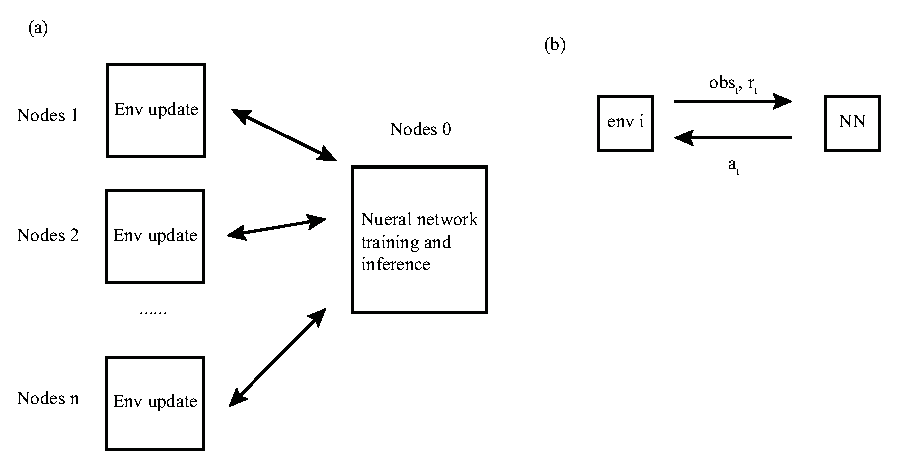
\includegraphics[]{./figures/schematics.eps}
    \caption{Illustration of general objective}
    \label{fig:comm}
\end{figure}


\section{Validation cases}\label{sec:case}

\section{Comparison}\label{sec:comp}
Using Proximal Policy Optimization (PPO) algorithm, on a same problem, train networks with four configurations, and compare their performance:

Activation function: $\tanh$, $\sin$

A separate actor and critic and combining actor and critic in a same neural network. 



\bibliography{reference.bib} 




\end{document}